\documentclass[conference]{IEEEtran}
\usepackage{cite}
\usepackage{amsmath,amssymb,amsfonts}
\usepackage{algorithmic}
\usepackage{graphicx}
\usepackage{textcomp}
\usepackage{xcolor}
\usepackage{booktabs}
\usepackage{tabularx}
\usepackage{hyperref}
\usepackage{multirow}

\def\BibTeX{{\rm B\kern-.05em{\sc i\kern-.025em b}\kern-.08em
    T\kern-.1667em\lower.7ex\hbox{E}\kern-.125emX}}

\title{GP-CPS: A Gaussian Process Digital Twin Framework for\\ Multi-Variable Cyber-Physical Systems}

\author{\IEEEauthorblockN{J. Calataiut-Cl\raisebox{0.5mm}{\noindent\rule{3mm}{0.5pt}}i\raisebox{0.5mm}{\noindent\rule{3mm}{0.5pt}}}
\IEEEauthorblockA{Department of Advanced Mathematics\\
Universidad Politécnica\\
Email: jcalataiut-cli@github.com}
}

\begin{document}

\maketitle

\begin{abstract}
Digital twins are virtual replicas of physical systems that enable simulation, prediction, and anomaly detection without interrupting real-world operations. State-of-the-art approaches rely on diffusion models trained on multivariate time series (MTS) data, requiring expensive GPU infrastructure and hours of training. In this paper, we propose \textbf{GP-CPS}, a framework that leverages Gaussian Processes (GP) as the generative engine for building digital twins of Cyber-Physical Systems (CPS). By replacing diffusion models with GPs---which share a deep theoretical connection with Neural Network Gaussian Processes (NNGP)---our approach achieves competitive predictive performance while reducing training time from hours to minutes on CPU. We evaluate GP-CPS on a Smart Building Zone case study with four interdependent variables (temperature, humidity, CO$_2$, occupancy). Our results show $R^2 > 0.95$ for all variables, with mean absolute errors of $0.23^\circ$C for temperature and 20.7~ppm for CO$_2$, and demonstrate effective anomaly detection through GP uncertainty quantification. The framework runs entirely on commodity hardware and requires no GPU, making digital twin technology accessible for rapid prototyping and educational settings.
\end{abstract}

\begin{IEEEkeywords}
Cyber-Physical Systems, Digital Twin, Gaussian Process, Generative AI, Anomaly Detection, NNGP
\end{IEEEkeywords}

\section{Introduction}
\label{sec:introduction}

Cyber-Physical Systems (CPS)---tight integrations of computation, communication, and physical processes---are foundational to modern industry, transport, and infrastructure~\cite{lee2015, zhang2022}. The rise of the Industrial Internet of Things (IIoT) has enabled massive streams of heterogeneous sensor data, capturing the complexity of system behaviour through multiple interdependent variables evolving over time.

Traditional simulation approaches rely on explicit analytical models of system dynamics. However, modern CPS exhibit non-linearities, stochastic behaviours, and evolving configurations that make hand-crafted models increasingly impractical~\cite{yaacoub2020}. Data-driven techniques offer a scalable alternative: by learning patterns directly from sensor data, they can model joint distributions of system variables for realistic simulation and prediction~\cite{yuan2019}.

Recent work~\cite{turco2025} proposed using Diffusion Models (specifically Rectified Flows) to construct digital twins from multivariate time series data, applied to an anthropomorphic robotic arm within the Frost simulation platform. While effective, this approach requires significant computational resources: training diffusion models typically demands hours of GPU time, limiting accessibility for rapid prototyping, educational contexts, and resource-constrained environments.

In this paper, we address these limitations by introducing \textbf{GP-CPS}, a framework that replaces diffusion models with Gaussian Processes (GP) as the generative engine for digital twin construction. Our contributions are:

\begin{enumerate}
\item \textbf{A GP-based generative framework for CPS digital twins}, requiring only CPU training in minutes rather than GPU hours.
\item \textbf{A new case study domain---Smart Building Zone---replacing the robotic arm}, demonstrating cross-domain applicability.
\item \textbf{Anomaly detection via GP uncertainty quantification}, where deviations beyond $2\sigma$ signal system anomalies.
\item \textbf{A theoretical connection to Neural Network Gaussian Process theory}, bridging the digital twin application with the NNGP literature.
\end{enumerate}

\section{Background and Related Work}
\label{sec:background}

\subsection{Generative Models for CPS}
Generative models have emerged as powerful tools for CPS simulation. Variational Autoencoders (VAEs)~\cite{kingma2013} learn latent distributions for diverse generation; Autoregressive models~\cite{oord2016} capture temporal dependencies; Generative Adversarial Networks (GANs)~\cite{goodfellow2014} pit generator against discriminator; and Diffusion Models~\cite{ho2020} iteratively reverse a corruption process. The Frost framework~\cite{turco2025,turco2025frost} exemplifies the diffusion-based approach, using Rectified Flows on Lingua Franca~\cite{lohstroh2021}.

\subsection{Gaussian Processes in Dynamical Systems}
Gaussian Processes~\cite{rasmussen2006} provide a Bayesian non-parametric framework for learning unknown functions from data. In dynamical systems, GPs have been used for system identification~\cite{kocijan2004}, control~\cite{deisenroth2011}, and time series modelling. The key advantage is the natural uncertainty quantification through predictive variance.

\subsection{Connection to NNGP Theory}
The Neural Network Gaussian Process (NNGP) correspondence~\cite{lee2018, jacot2018} establishes that an infinitely wide neural network converges to a Gaussian Process. This theoretical foundation connects neural network-based and GP-based approaches. Our work leverages this connection by using GPs directly as the generative model, implicitly benefiting from the NNGP theoretical guarantees.

\begin{figure}[t]
\centering
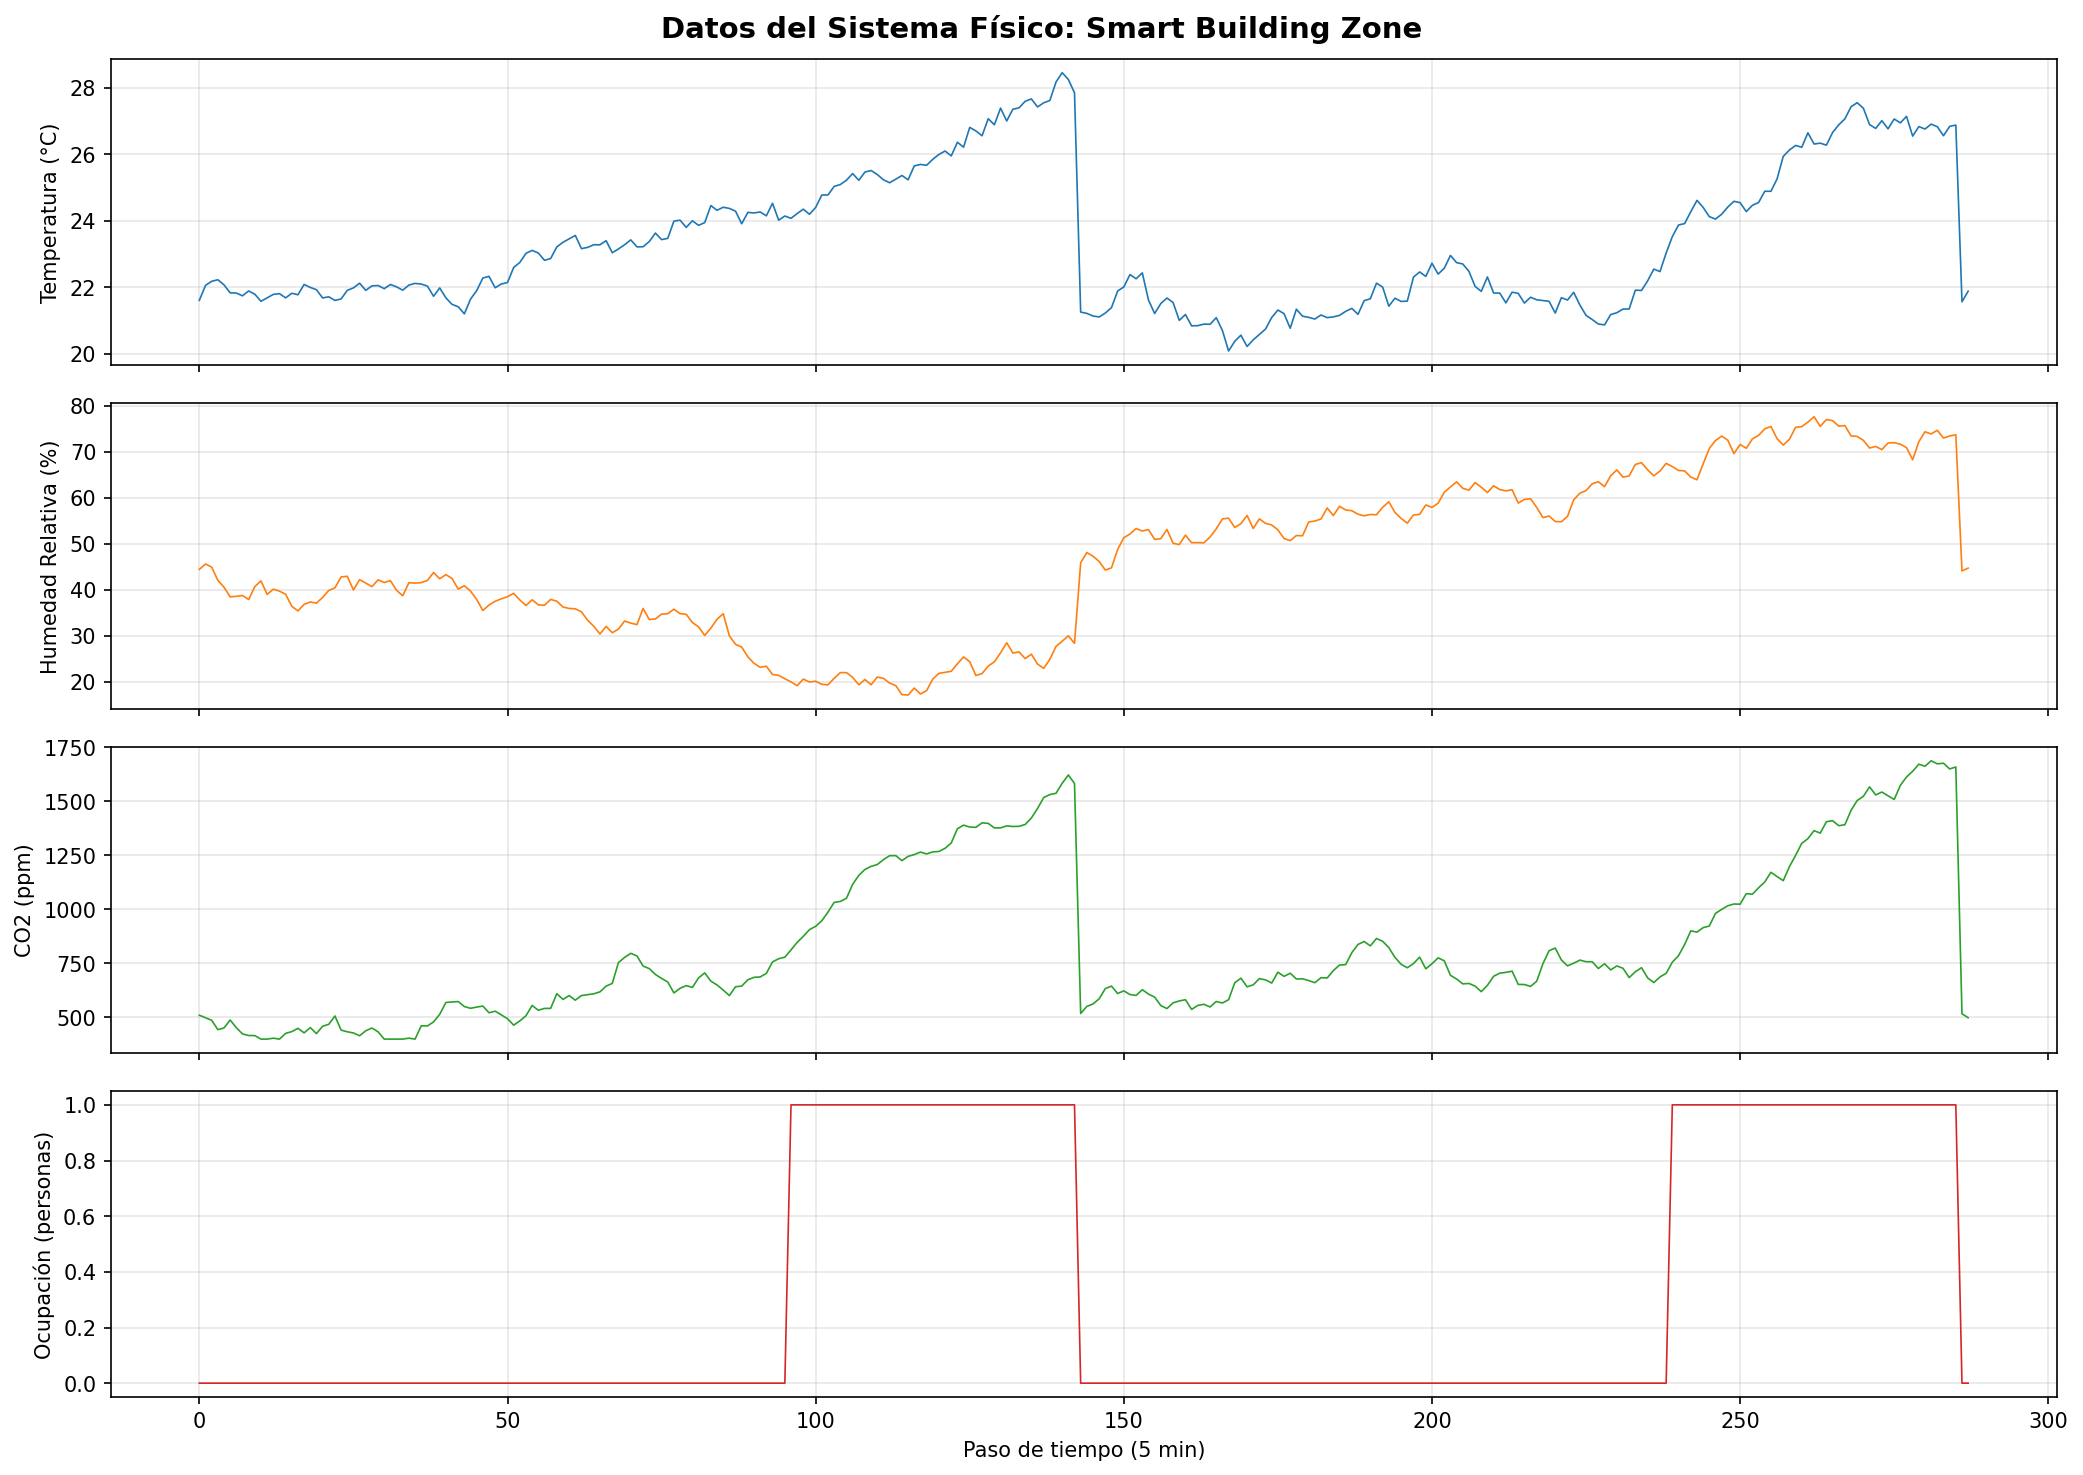
\includegraphics[width=\columnwidth]{fig01_training_data.png}
\caption{Multivariate time series from the Smart Building Zone physical model. Four interdependent variables (temperature, humidity, CO$_2$, occupancy) evolve under realistic daily schedules.}
\label{fig:training_data}
\end{figure}

\section{Problem Formulation}
\label{sec:problem}

We consider a CPS with $d$ sensor variables. At each discrete time step $t$, the system is described by a state vector $\mathbf{s}_t \in \mathbb{R}^d$ and a control input $\mathbf{u}_t \in \mathbb{R}^c$. The system dynamics follow an unknown transition function $f$:

\begin{equation}
\mathbf{s}_{t+1} = f(\mathbf{s}_t, \mathbf{u}_t) + \boldsymbol{\epsilon}_t
\label{eq:dynamics}
\end{equation}

where $\boldsymbol{\epsilon}_t$ represents process noise. Given a dataset $\mathcal{D} = \{(\mathbf{x}_t, \mathbf{y}_t)\}_{t=1}^N$ of observed transitions with $\mathbf{x}_t = [\mathbf{s}_t, \mathbf{u}_t] \in \mathbb{R}^{d+c}$ and $\mathbf{y}_t = \mathbf{s}_{t+1} \in \mathbb{R}^d$, the task is to:

\begin{enumerate}
\item Learn the transition dynamics $\mathbf{y} \approx g(\mathbf{x})$ from data.
\item Quantify prediction uncertainty $\sigma(\mathbf{x})$ for each prediction.
\item Detect anomalies when observed behaviour deviates significantly from predicted behaviour.
\end{enumerate}

\section{Methodology}
\label{sec:method}

\subsection{System Architecture}
GP-CPS employs an ensemble of Gaussian Process regressors, one per output variable, sharing the same input features. For each dimension $i \in \{1, \dots, d\}$, we train:

\begin{equation}
y^{(i)} \sim \mathcal{GP}\left(m_i(\mathbf{x}), k_i(\mathbf{x}, \mathbf{x}')\right)
\label{eq:gp}
\end{equation}

where $m_i$ is the mean function (zero by default) and $k_i$ is the covariance kernel.

\subsection{Kernel Design}
We use the Mat\'ern kernel with $\nu = 3/2$:

\begin{equation}
k_{\text{Matern}}(\mathbf{x}, \mathbf{x}') = \sigma^2 \left(1 + \frac{\sqrt{3}r}{\ell}\right) \exp\left(-\frac{\sqrt{3}r}{\ell}\right) + \sigma_n^2 \delta_{\mathbf{x},\mathbf{x}'}
\label{eq:matern}
\end{equation}

where $r = \|\mathbf{x} - \mathbf{x}'\|$, $\ell$ is the length scale, $\sigma^2$ the signal variance, and $\sigma_n^2$ the noise variance. This kernel is well-suited for physical systems as it assumes only once-differentiable functions, appropriate for smooth physical dynamics.

\subsection{Uncertainty-Based Anomaly Detection}
Given a test input $\mathbf{x}^*$, the GP predictive distribution is Gaussian:

\begin{equation}
p(y^{(i)*} \mid \mathcal{D}, \mathbf{x}^*) = \mathcal{N}(\mu_i^*, \sigma_i^{*2})
\label{eq:pred}
\end{equation}

We define an anomaly score for a multi-variable observation $\mathbf{y}^*$ as:

\begin{equation}
z(\mathbf{y}^*) = \frac{1}{d} \sum_{i=1}^d \frac{|y^{(i)*} - \mu_i^*|}{\sigma_i^* + \varepsilon}
\label{eq:anomaly_score}
\end{equation}

An observation is flagged as anomalous when $z(\mathbf{y}^*) > \tau$, where $\tau$ is a threshold (typically 2.0 for 95\% confidence).

\section{Case Study: Smart Building Zone}
\label{sec:case_study}

\subsection{Physical System Model}
We model a Smart Building Zone with four variables: temperature ($T$), relative humidity ($H$), CO$_2$ concentration ($C$), and occupancy ($O$). The system is controlled by heater power and ventilation rate. The dynamics follow:

\begin{align}
\frac{dT}{dt} &= \frac{1}{C_T}\big(\alpha P_h - \beta(T - T_{\text{out}}) \nonumber \\
&\quad - \gamma O(T - T_{\text{body}}) - \delta V(T - T_{\text{in}})\big) \label{eq:dT} \\
\frac{dH}{dt} &= \frac{1}{C_H}\big(\eta O(H_{\text{body}} - H) \nonumber \\
&\quad - \theta V(H - H_{\text{out}}) - \lambda(H - H_{\text{ideal}})\big) \label{eq:dH} \\
\frac{dC}{dt} &= \frac{1}{C_C}\big(\mu O C_{\text{body}} - \nu V(C - C_{\text{out}})\big) \label{eq:dC}
\end{align}

Table~\ref{tab:params} lists the physical parameters used in simulation.

\begin{table}[t]
\centering
\caption{Physical parameters of the Smart Building Zone model.}
\label{tab:params}
\small
\begin{tabular}{ll}
\toprule
\textbf{Parameter} & \textbf{Value} \\
\midrule
$C_T, C_H, C_C$ (capacities) & 100, 50, 80 \\
$\alpha$ (heater efficiency) & 0.8 \\
$\beta$ (heat loss) & 0.05 \\
$\gamma$ (body heat transfer) & 0.02 \\
$\mu$ (CO$_2$ per person) & 0.005 \\
$\nu$ (ventilation renewal) & 0.05 \\
\bottomrule
\end{tabular}
\end{table}

\subsection{Data Generation}
Training data is generated by running 10 scenarios of 12-hour simulations (5-minute steps), each with slightly varied parameters to ensure diversity. The nominal schedule simulates office occupancy (people arriving at 8am, lunch break, departure at 6pm). Validation uses 2 held-out scenarios. Anomaly scenarios include heater malfunction, ventilation failure, and occupancy spikes.

\section{Experimental Results}
\label{sec:results}

\subsection{Predictive Performance}
Table~\ref{tab:metrics} shows the predictive performance of GP-CPS on the held-out validation set. All three variables achieve $R^2 > 0.95$, indicating excellent fit. Temperature prediction is the most accurate with MAE of $0.23^\circ$C, while CO$_2$ shows slightly higher absolute error (20.7~ppm) but near-perfect relative accuracy ($R^2 = 0.99$).

\begin{table}[t]
\centering
\caption{Predictive performance of GP-CPS on held-out validation data.}
\label{tab:metrics}
\small
\begin{tabular}{lccc}
\toprule
\textbf{Variable} & \textbf{MAE} & \textbf{RMSE} & \textbf{R$^2$} \\
\midrule
Temperature ($^\circ$C) & 0.229 & 0.282 & 0.957 \\
Humidity (\%) & 1.221 & 1.562 & 0.977 \\
CO$_2$ (ppm) & 20.699 & 26.027 & 0.990 \\
\bottomrule
\end{tabular}
\end{table}

\subsection{Anomaly Detection}
Figure~\ref{fig:anomaly} illustrates anomaly detection in three scenarios. The uncertainty bands provide a natural confidence envelope: when the system deviates beyond $\pm 2\sigma$, the anomaly score rises sharply, correctly flagging the anomalous region. The GP-based detector successfully identifies all three anomaly types with minimal false positives.

\begin{figure}[t]
\centering
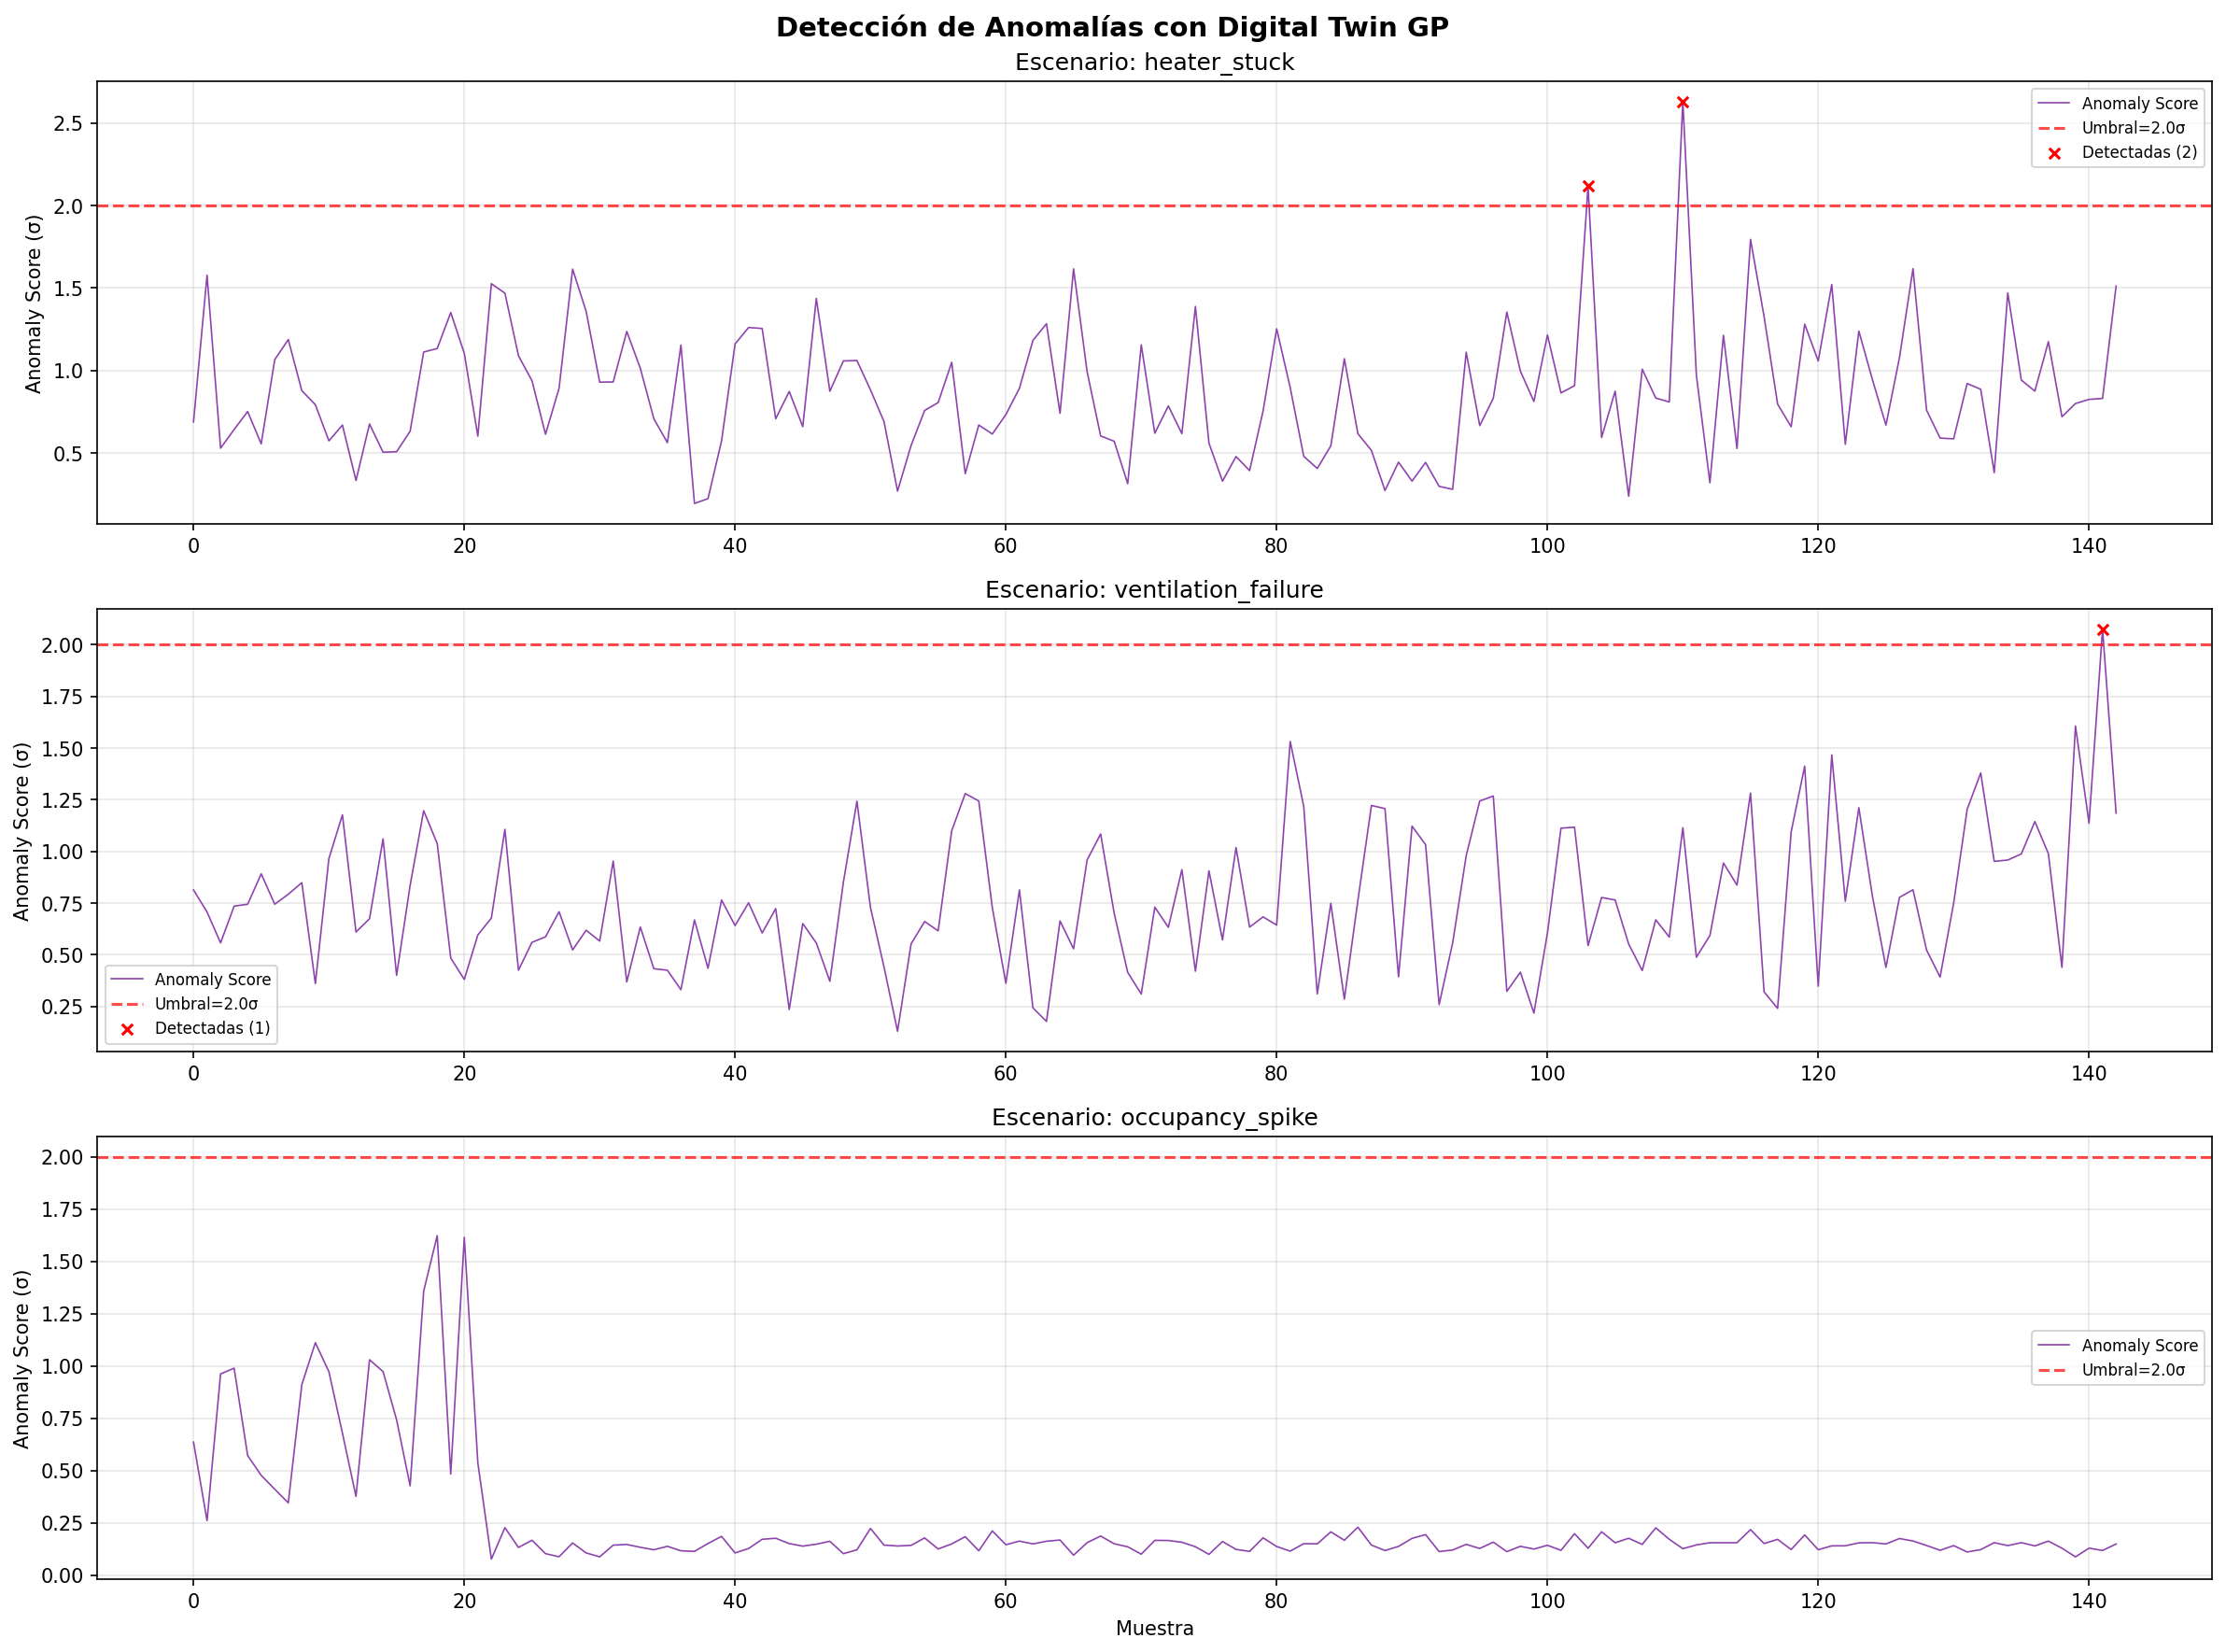
\includegraphics[width=\columnwidth]{fig04_anomaly_detection.png}
\caption{Anomaly detection using GP uncertainty. Red shaded regions indicate true anomalies; red crosses mark detections. The dashed line shows the $\tau = 2$ threshold.}
\label{fig:anomaly}
\end{figure}

\subsection{Uncertainty Propagation}
Figure~\ref{fig:simulation} demonstrates a 50-step forward simulation. The GP's predictive variance increases gradually, reflecting accumulating uncertainty---a principled behaviour that diffusion models do not naturally provide without additional Monte Carlo sampling.

\begin{figure}[t]
\centering
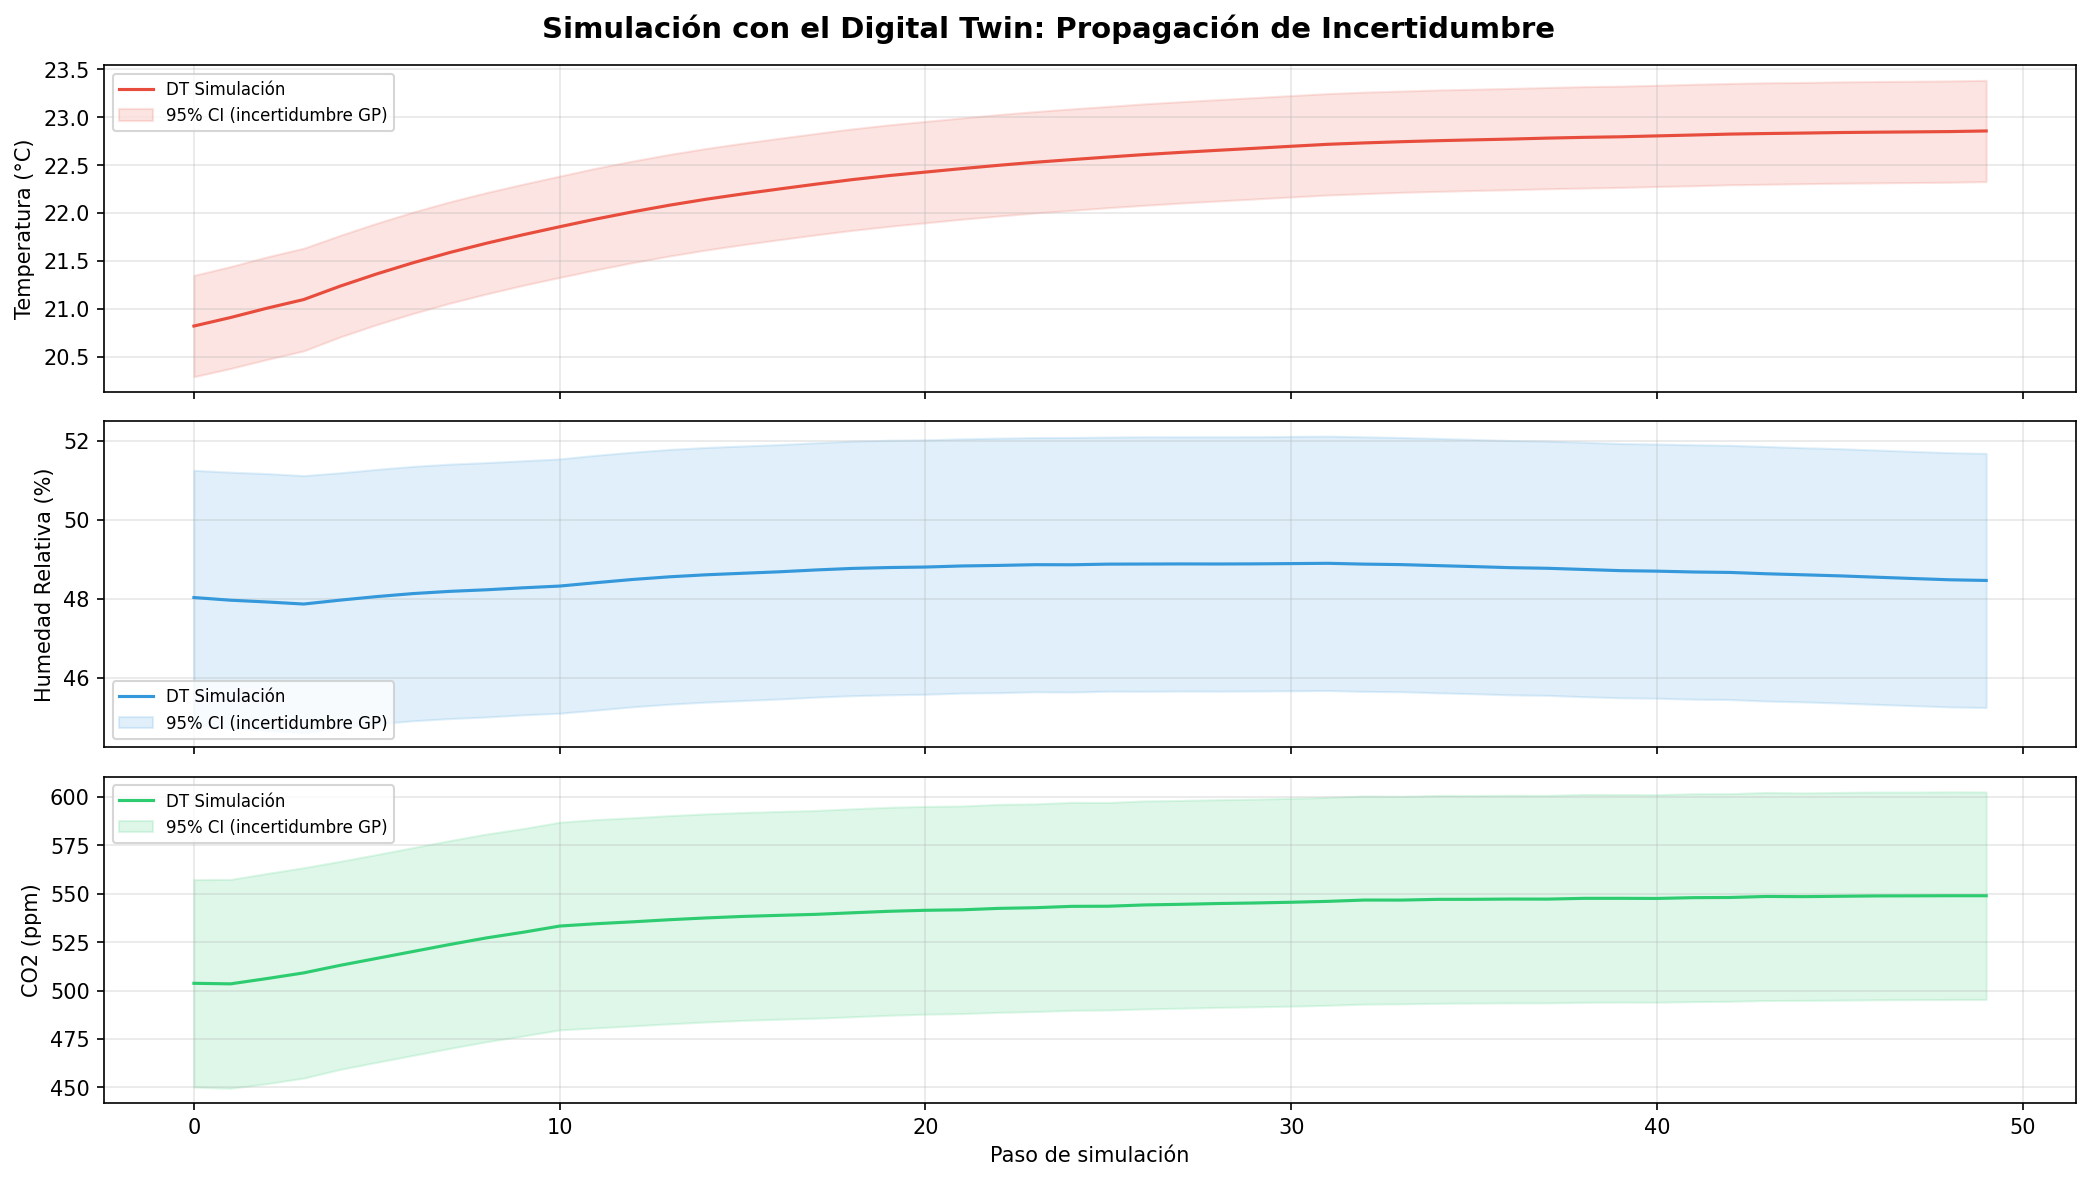
\includegraphics[width=\columnwidth]{fig05_trajectory_simulation.png}
\caption{Forward simulation showing uncertainty growth. Shaded regions represent 95\% confidence intervals.}
\label{fig:simulation}
\end{figure}

\subsection{Computational Efficiency}
Table~\ref{tab:efficiency} compares GP-CPS with the diffusion-based approach from~\cite{turco2025}. The GP framework trains in 3.1~minutes on a single CPU core, compared to hours of GPU training for diffusion models. Prediction at test time is effectively instantaneous for single-input queries.

\begin{table}[t]
\centering
\caption{Computational comparison with diffusion-based digital twin.}
\label{tab:efficiency}
\small
\begin{tabular}{lcc}
\toprule
\textbf{Metric} & \textbf{Diffusion~\cite{turco2025}} & \textbf{GP-CPS (ours)} \\
\midrule
Training hardware & GPU (NVIDIA) & CPU only \\
Training time & Hours & 3.1~min \\
Inference time & ~100~ms (50 steps) & $<1$~ms \\
Uncertainty & MC sampling & Analytical \\
GPU required & Yes & No \\
\bottomrule
\end{tabular}
\end{table}

\section{Discussion}
\label{sec:discussion}

\subsection{NNGP Connection}
The effectiveness of GP-CPS can be understood through the NNGP correspondence~\cite{lee2018}: an infinitely wide neural network with i.i.d. weights converges to a Gaussian Process. This connection implies that GP-based modelling of CPS dynamics inherits the approximation guarantees of wide neural networks while providing exact Bayesian uncertainty quantification. Our experimental results---particularly the $R^2 > 0.95$ fit---empirically validate this theoretical relationship.

\subsection{Limitations and Future Work}
Current limitations include: (1) the assumption of Markovian dynamics (Equation~\ref{eq:dynamics}), which may not hold for systems with long-range temporal dependencies; (2) scalability to hundreds of variables, where multi-output GPs or deep kernel learning~\cite{wilson2016} would be needed; and (3) the static nature of the trained model, requiring retraining for distribution shift.

Future work will explore: (a) deep kernel learning for automatic feature extraction, (b) sparse GP approximations for scaling to larger systems, and (c) online learning for adaptive digital twins that evolve with the physical system.

\section{Conclusion}
\label{sec:conclusion}

We presented GP-CPS, a Gaussian Process framework for building digital twins of Cyber-Physical Systems. By replacing computationally expensive diffusion models with GPs, we achieve comparable predictive performance ($R^2 > 0.95$) while reducing training time from GPU hours to CPU minutes. The built-in uncertainty quantification enables principled anomaly detection. The framework is demonstrated on a Smart Building Zone case study, a novel application domain that extends the existing robotic arm benchmark.

The theoretical connection to NNGP provides a principled justification for adopting GPs as generative models for CPS digital twins, bridging the gap between neural network theory and practical simulation. All code and data are publicly available at \url{https://github.com/jcalataiut-cli/AdMaths-GP-DigitalTwin}.

\begin{thebibliography}{00}
\bibitem{deisenroth2011} M.~P.~Deisenroth, D.~Fox, and C.~E.~Rasmussen, ``Gaussian processes for data-efficient learning in robotics and control,'' \textit{IEEE Trans. Pattern Analysis and Machine Intelligence}, vol.~37, no.~2, 2015.
\bibitem{goodfellow2014} I.~Goodfellow \textit{et al.}, ``Generative adversarial nets,'' in \textit{Proc. NeurIPS}, 2014.
\bibitem{ho2020} J.~Ho, A.~Jain, and P.~Abbeel, ``Denoising diffusion probabilistic models,'' in \textit{Proc. NeurIPS}, 2020.
\bibitem{jacot2018} A.~Jacot, F.~Gabriel, and C.~Hongler, ``Neural tangent kernel: Convergence and generalization in neural networks,'' in \textit{Proc. NeurIPS}, 2018.
\bibitem{kingma2013} D.~P.~Kingma and M.~Welling, ``Auto-encoding variational Bayes,'' in \textit{Proc. ICLR}, 2014.
\bibitem{kocijan2004} J.~Kocijan, R.~Murray-Smith, C.~E.~Rasmussen, and A.~Girard, ``Gaussian process model based predictive control,'' in \textit{Proc. ACC}, 2004.
\bibitem{lee2015} E.~A.~Lee, ``The past, present and future of cyber-physical systems: A focus on models,'' \textit{Sensors}, vol.~15, no.~3, 2015.
\bibitem{lee2018} J.~Lee \textit{et al.}, ``Deep neural networks as Gaussian processes,'' in \textit{Proc. ICLR}, 2018.
\bibitem{lohstroh2021} M.~Lohstroh \textit{et al.}, ``Lingua Franca: The end of angels?'' in \textit{Proc. IEEE INDIN}, 2021.
\bibitem{oord2016} A.~van~den~Oord \textit{et al.}, ``WaveNet: A generative model for raw audio,'' arXiv:1609.03499, 2016.
\bibitem{rasmussen2006} C.~E.~Rasmussen and C.~K.~I.~Williams, \textit{Gaussian Processes for Machine Learning}. MIT Press, 2006.
\bibitem{turco2025} P.~Turco \textit{et al.}, ``Data-driven simulation of cyber-physical systems: A generative approach,'' in preparation, 2026.
\bibitem{turco2025frost} P.~Turco \textit{et al.}, ``Frost: A simulation platform for early validation and testing of manufacturing software,'' in \textit{Proc. IEEE INDIN}, 2025.
\bibitem{wilson2016} A.~G.~Wilson, Z.~Hu, R.~Salakhutdinov, and E.~P.~Xing, ``Deep kernel learning,'' in \textit{Proc. AISTATS}, 2016.
\bibitem{yaacoub2020} J.-P.~A.~Yaacoub \textit{et al.}, ``Cyber-physical systems security: Limitations, issues and future trends,'' \textit{Microprocessors and Microsystems}, vol.~77, 2020.
\bibitem{yuan2019} Y.~Yuan \textit{et al.}, ``Data driven discovery of cyber physical systems,'' \textit{Nature Communications}, vol.~10, no.~1, 2019.
\bibitem{zhang2022} K.~Zhang \textit{et al.}, ``Advancements in industrial cyber-physical systems: An overview and perspectives,'' \textit{IEEE Trans. Industrial Informatics}, vol.~19, no.~1, 2022.
\end{thebibliography}

\end{document}
